%%%%%%%%%%%%%%%%%%%%%%%%%%%%%%%%%%%%%%%%%%%%%%%%%%%%%%%%%%%%%%%%%%%%%%%%%%%%%%%%%%
\begin{frame}[fragile]\frametitle{}

\begin{center}
{\Large Project: Sentiment Analysis of Twitter Posts on Chennai Floods using Python}
\end{center}
\end{frame}

%%%%%%%%%%%%%%%%%%%%%%%%%%%%%%%%%%%%%%%%%%%%%%%%%%%%%%%%%%%%%%%%%%%%%%%%%%%%%%%%%%
\begin{frame}[fragile]\frametitle{Introduction}
  \begin{itemize}
  \item The best way to learn data science is to do data science.
  \item Came across a study on sentiment analysis of Chennai Floods on Analytics Vidhya. https://www.analyticsvidhya.com/blog/2016/07/capstone-project/
  \item Decided to perform sentiment analysis of the same study using Python.
  \item Original study about crisis of Chennai floods (https://www.analyticsvidhya.com/blog/2016/07/capstone-project/). 
  \item This study was done on a set of social interactions limited to the first two days of Chennai Floods in December 2015.
  \end{itemize}
\end{frame}

%%%%%%%%%%%%%%%%%%%%%%%%%%%%%%%%%%%%%%%%%%%%%%%%%%%%%%%%%%%%%%%%%%%%%%%%%%%%%%%%%%
\begin{frame}[fragile]\frametitle{Objective}
  \begin{itemize}
  \item Understand the different subjects of interactions during the floods using Python. 
  \item Grouping similar messages together with emphasis on predominant themes (rescue, food, supplies, ambulance calls) can help government and other authorities to act in the right manner during the crisis time.
  \end{itemize}
\end{frame}

%%%%%%%%%%%%%%%%%%%%%%%%%%%%%%%%%%%%%%%%%%%%%%%%%%%%%%%%%%%%%%%%%%%%%%%%%%%%%%%%%%
\begin{frame}[fragile]\frametitle{Building Corpus}
  \begin{itemize}
  \item A typical tweet is mostly a text message within limit of 140 characters. 
  \item \#hashtags convey subject of the tweet whereas @user seeks attention of that user. 
  \item Forwarding is denoted by `rt' (retweet) and is a measure of its popularity. 
  \item One can like a tweet by making it `favorite'.
  \item About 6000 twits were collected with `\#ChennaiFloods' hashtag and between 1st and 2nd Dec 2015.  
  \item Jefferson's GetOldTweets utility (got) was used in Python 2.7 to collect the older tweets.
  \item One can store the tweets either in a csv file or to a database like MongoDb to be used for further processing.
  \end{itemize}
\end{frame}

%%%%%%%%%%%%%%%%%%%%%%%%%%%%%%%%%%%%%%%%%%%%%%%%%%%%%%%%%%%%%%%%%%%%%%%%%%%%%%%%%%
\begin{frame}[fragile]\frametitle{Building Corpus}
  \begin{lstlisting}
import got, codecs
from pymongo import MongoClient 
client = MongoClient('localhost', 27017)
db = client['twitter_db']
collection = db['twitter_collection']
tweetCriteria = 
got.manager.TweetCriteria().setQuerySearch('ChennaiFloods').setSince("2015-12-01").setUntil("2015-12-02").setMaxTweets(6000)
def streamTweets(tweets):
   for t in tweets:
      obj = {"user": t.username, "retweets": t.retweets, "favorites":  
            t.favorites, "text":t.text,"geo": t.geo,"mentions": 
            t.mentions, "hashtags": t.hashtags,"id": t.id,
            "permalink": t.permalink,}
      tweetind = collection.insert_one(obj).inserted_id
got.manager.TweetManager.getTweets(tweetCriteria, streamTweets)
  \end{lstlisting}
\end{frame}

%%%%%%%%%%%%%%%%%%%%%%%%%%%%%%%%%%%%%%%%%%%%%%%%%%%%%%%%%%%%%%%%%%%%%%%%%%%%%%%%%%
\begin{frame}[fragile]\frametitle{Building Corpus}
Tweets stored in MongoDB can be accessed from another python script. 
  \begin{lstlisting}
import pandas as pd
from pymongo import MongoClient
client = MongoClient ('localhost', 27017)
db = client ['twitter_db']
collection = db ['twitter_collection']
df=pd.DataFrame(list(collection.find()))
  \end{lstlisting}
  \begin{center}
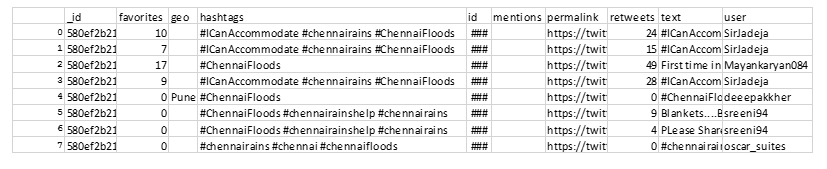
\includegraphics[width=\linewidth,keepaspectratio]{tw1}
\end{center}
\end{frame}

%%%%%%%%%%%%%%%%%%%%%%%%%%%%%%%%%%%%%%%%%%%%%%%%%%%%%%%%%%%%%%%%%%%%%%%%%%%%%%%%%%
\begin{frame}[fragile]\frametitle{Data Exploration}
Once in dataframe format, it is easier to explore the data:
  \begin{lstlisting}
hashtags = []
for hs in df["hashtags"]: # Each entry may contain multiple hashtags. Split.
       hashtags += hs.split(" ")
fdist1 = FreqDist(hashtags)
fdist1.plot(10)
  \end{lstlisting}
  \begin{center}
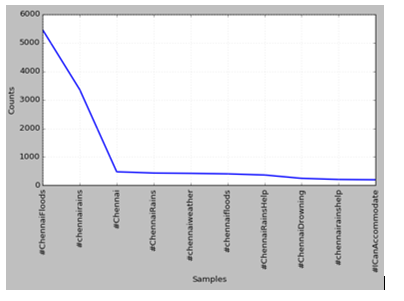
\includegraphics[width=0.3\linewidth,keepaspectratio]{tw2}
\end{center}
As seen in the study the most used tags were ``\#chennairains'', ``\#ICanAccommodate'', apart from the original query tag ``\#ChennaiFloods''.
\end{frame}


%%%%%%%%%%%%%%%%%%%%%%%%%%%%%%%%%%%%%%%%%%%%%%%%%%%%%%%%%%%%%%%%%%%%%%%%%%%%%%%%%%
\begin{frame}[fragile]\frametitle{Text Pre-processing}
All tweets are processed to remove unnecessary things like links, non-English words, stopwords, punctuation's, etc.
  \begin{lstlisting}
def process_tweet_text(tweet):
   if tweet.startswith('@null'):
       return "[Tweet not available]"
   tweet = re.sub(r'\$\w*','',tweet) # Remove tickers
   tweet = re.sub(r'https?:\/\/.*\/\w*','',tweet) # Remove hyperlinks
   tweet = re.sub(r'['+string.punctuation+']+', ' ',tweet) 
   twtok = TweetTokenizer(strip_handles=True, reduce_len=True)
   tokens = twtok.tokenize(tweet)
   tokens = [i.lower() for i in tokens if i not in stopwords and len(i) > 2 and  i in english_vocab]
   return tokens
  \end{lstlisting}
The word list generated looks like: [`time', `history', `temple', `closed', `due', `pic', `twitter', `havoc', `incessant', \ldots]
\end{frame}

%%%%%%%%%%%%%%%%%%%%%%%%%%%%%%%%%%%%%%%%%%%%%%%%%%%%%%%%%%%%%%%%%%%%%%%%%%%%%%%%%%
\begin{frame}[fragile]\frametitle{Text Exploration}
The words are plotted again to find the most frequently used terms. A few simple words repeat more often than others: 'help', `people', `stay', 'safe', etc.
These are immediate reactions and responses to the crisis.
\lstinline|[(`twitter', 1026), (`pic', 1005), (`help', 569), (`people', 429), (`safe', 274)]|
Some infrequent terms are \lstinline|[(`fit', 1), (`bible', 1), (`disappear', 1), (`regulated', 1), (`doom', 1)].|
  \begin{center}
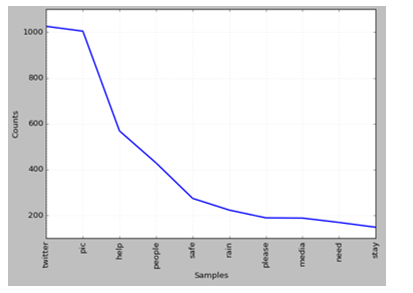
\includegraphics[width=0.5\linewidth,keepaspectratio]{tw3}
\end{center}
\end{frame}


%%%%%%%%%%%%%%%%%%%%%%%%%%%%%%%%%%%%%%%%%%%%%%%%%%%%%%%%%%%%%%%%%%%%%%%%%%%%%%%%%%
\begin{frame}[fragile]\frametitle{Text Exploration}
Collocations are the words found together:  bi-grams (two words together) or phrases like trigrams (3 words) or n-grams (n words).
  \begin{lstlisting}
from nltk.collocations import *
bigram_measures = nltk.collocations.BigramAssocMeasures()
finder = BigramCollocationFinder.from_words(words, 5)
finder.apply_freq_filter(5)
print(finder.nbest(bigram_measures.likelihood_ratio, 10))
  \end{lstlisting}
  Most frequently appearing Bigrams are:
  \begin{lstlisting}
[(`pic', `twitter'), (`lady', `labour'), (`national', `media'), (`pani', `pani'), (`team', `along'), (`stay', `safe'), (`rescue', `team'), (`beyond', `along'), (`team', `beyond'), (`rescue', `along')]
  \end{lstlisting}
These depict the disastrous situation, like ``stay safe'', ``rescue team'', even a commonly used Hindi phrase ``pani pani'' (lots of water).
\end{frame}

%%%%%%%%%%%%%%%%%%%%%%%%%%%%%%%%%%%%%%%%%%%%%%%%%%%%%%%%%%%%%%%%%%%%%%%%%%%%%%%%%%
\begin{frame}[fragile]\frametitle{Clustering}
  \begin{itemize}
  \item In such crisis situations, lots of similar tweets are generated.
  \item They can be grouped together in clusters based on closeness or `distance' amongst them. 
  \item TF-IDF method is used to vectorize the tweets and then cosine distance is measured to assess the similarity.
  \end{itemize}
  \begin{center}
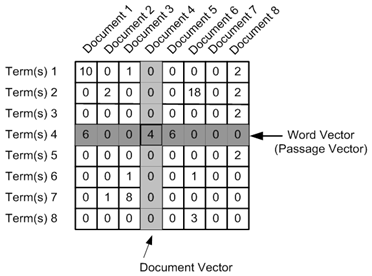
\includegraphics[width=0.5\linewidth,keepaspectratio]{tw4}
\end{center}
\end{frame}

%%%%%%%%%%%%%%%%%%%%%%%%%%%%%%%%%%%%%%%%%%%%%%%%%%%%%%%%%%%%%%%%%%%%%%%%%%%%%%%%%%
\begin{frame}[fragile]\frametitle{Clustering}
  \begin{itemize}
  \item Vectorization is done using 1-3 n-grams, meaning phrases with 1,2,3 words are used to compute frequencies, i.e. TF IDF values.
  \item One can get cosine similarity amongst tweets/documents as well.
    \end{itemize}
  \begin{lstlisting}
from sklearn.feature_extraction.text import TfidfVectorizer  

tfidf_vectorizer = TfidfVectorizer(use_idf=True, ngram_range=(1,3))  
tfidf_matrix = tfidf_vectorizer.fit_transform(cleaned_tweets)  
feature_names = tfidf_vectorizer.get_feature_names() # num phrases  

from sklearn.metrics.pairwise import cosine_similarity  
dist = 1 - cosine_similarity(tfidf_matrix)  
print(dist) 
  \end{lstlisting}
\end{frame}

%%%%%%%%%%%%%%%%%%%%%%%%%%%%%%%%%%%%%%%%%%%%%%%%%%%%%%%%%%%%%%%%%%%%%%%%%%%%%%%%%%
\begin{frame}[fragile]\frametitle{Clustering}
  \begin{itemize}
  \item K-means clustering algorithm is used to group tweets into choosen number (say, 3) of groups.
\item The output shows 3 clusters, with following number of tweets in respective clusters.
    \end{itemize}
  \begin{lstlisting}
from sklearn.cluster 
import KMeans  

num_clusters = 3  
km = KMeans(n_clusters=num_clusters)  
km.fit(tfidf_matrix)  

clusters = km.labels_.tolist()  

df['ClusterID'] = clusters  
print(df['ClusterID'].value_counts())
  \end{lstlisting}
    \begin{center}
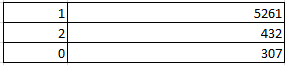
\includegraphics[width=0.4\linewidth,keepaspectratio]{tw5}
\end{center}
\end{frame}

%%%%%%%%%%%%%%%%%%%%%%%%%%%%%%%%%%%%%%%%%%%%%%%%%%%%%%%%%%%%%%%%%%%%%%%%%%%%%%%%%%
\begin{frame}[fragile]\frametitle{Clustering}
The top words used in each cluster can be computed by as follows:
  \begin{lstlisting}
#sort cluster centers by proximity to centroid
order_centroids = km.cluster_centers_.argsort()[:, ::-1]
for i in range(num_clusters):
    print("Cluster {} : Words :".format(i))
    for ind in order_centroids[i, :10]: 
        print(' %s' % feature_names[ind])
  \end{lstlisting}
  The result is:
  \begin{itemize}
  \item 
    Cluster 0: Words: show mercy please people rain
  \item     Cluster 1: Words: pic twitter zoo wall broke ground saving guilty water growing
  \item     Cluster 2: Words: help people pic twitter safe open rain share please
    \end{itemize}
        It is clear from the words associated with the topics that they represent certain sentiments. Cluster 0 is about Requests, Custer 1 is about Accidents, Custer 2 is about Communication, etc.
\end{frame}

